\documentclass{resume} % Use the custom resume.cls style

\usepackage[left=0.75in,top=0.6in,right=0.75in,bottom=0.6in]{geometry} % Document margins
\usepackage{graphicx}
%\graphicspath{{images/}}
\name {Vikas M} % Your name
\address {S/O Manjunatha.N,C/O Sri Nandi Medicals,T.K Road,Old Town Bhadravathi-577301}
\address{Shimoga(Dist.) Karnataka (S)} % Your address
\address{+919741641879 \\ vikasmdevang@gmail.com} % Your phone number and email

\begin{document}
\begin{figure}[h]

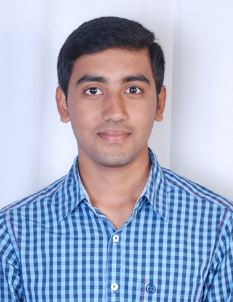
\includegraphics[height=4cm,width=3cm]{vikky.jpg}\\
%\caption{Block Diagram of Remote Automation and Data monitoring of Irrigation System}\label{fig 2.1}
\end{figure}
\begin{rSection}{Career Objective}
To obtain a Position in Technology field specifically dealing with programming and developments.
\end{rSection}

\begin{rSection}{Education}
\begin{center}
	\begin{tabular}{||c|c|c|c|c||}
		\hline\hline
		\bf Examination & \bf Institute & \bf University & \bf Year & \bf Performance \\
		\hline\hline
	    B.E(ECE) & JNN College of Engineering & VTU & 2015 & 70.21\% \\
		\hline
		II PUC/XII & Sri Aurobindo PU College & Karnataka State Board & 2011 & 86.83\% \\
		\hline
		SSLC/X & Poorna Pragna Education Centre & Karnataka State Board & 2009 & 93.76\% \\
		\hline\hline
		
		
	\end{tabular}
\end{center}

\end{rSection}

\begin{rSection}{Projects}

\begin{enumerate}

\item \begin{rSubsection}{Remote Automation in Agriculture}{April, 2015}{Electronics \& Communication}{JNNCE,Shivamogga}
\item Automating a agricultural field by sending an SMS to the system which checks the various parameters such as availabilty of ground water,Soil moisture level,Three phase availability and whether its raining are not and then Switches on the MOTOR if all the parameters are satisfied.
\end{rSubsection}

\item \begin{rSubsection}{Workshops Conducted}{July, 2014}{Electronics \& Communication}{JNNCE,Shivamogga}
\item Conducted �Hobby Project Hands on Workshop� for 3rd Sem EC students.
\item Conducted �MSP 430 Microcontroller Hands on Workshop� for 5th Sem EC students of our college.
\end{rSubsection}

\end{enumerate}
\end{rSection}


\begin{rSection}{Training and Internship}
	\begin{itemize}
		\item \begin{rSubsection}{Vocational Training on Telecom Technologies}{January, 2014}{Electronics \& Communication}{BSNL,Shivamogga}
            \item Successfully completed the communication training in BSNL.
			\end{rSubsection}
		\item Successfully completed 3 days of Workshop on �Introduction to Computer Hardware and Networking� conducted by Department of EC of our college.
        \item Presently doing Internship at IIT BOMBAY,Mumbai on Robotics and Embedded C.
	\end{itemize}
\end{rSection}

\begin{rSection}{Research Publication}
	\begin{enumerate}
		\item Read a research paper on "Spintronics" as a part of an academic activity.
		\item No research paper publication yet
	\end{enumerate}
\end{rSection}

\begin{rSection}{Technical Skills}
\begin{itemize}
		\item Coding and Debugging
		\item Programming and Problem Solving
		\item Testing and TroubleShooting
		\item Robotics
\end{itemize}
\end{rSection}

\begin{rSection}{Soft Skills}
	\begin{enumerate}
		\item C++, C, Embedded C
		\item Latex
		\item Cadence
		\item Matlab
		
	\end{enumerate}
\end{rSection}
\begin{rSection}{Extra-Curricular Activities}
	\begin{itemize}
        \item Participated in a National Level Robotics Challenge organised by IIT Bombay and grabbed 1st Place among 52 teams.
        \item Won first prize in National level Project Competition conducted by IETE at Amrutha College of Engineering,Coimbatore.
		\item Won Second Prize in Circuitrix Competition at
              Techzone 2K12,a State Level Technical Symposium held in our College.
        \item Participated in National Level Technical Paper Presentation 'E-Manthana' held in AIT College Chickmagalur.

	\end{itemize}
\end{rSection}

\begin{rSection}{Co-Curricular activities}
	\begin{enumerate}
		\item Won Second Prize in Robowars competition held in our College.
\item Was a Runner Up in Inter Poorna Prajna Volley Ball Competition,held in Yelahanka New Town,Bangalore.
\item Participated in District Level Scouts and Guides Training held in Shimoga.
	\end{enumerate}
\end{rSection}

\begin{rSection}{Hobbies and Interest}
    \begin{itemize}
    \item Listening to Music
    \item Playing Cricket
    \item Playing Carrom
    \end{itemize}    
\end{rSection}

\newpage

\begin{rSection}{Personal Information}
	\item \textbf{Father�s Name:} Manjunatha.N
	\item \textbf{Mother�s Name: } Pushpavathi.R
	\item \textbf{Sex:} Male
	\item \textbf{Date of Birth:} 27th December,1992
	\item \textbf{Nationality: } Hindu
	\item \textbf{Marital Status:}	Single
\end{rSection}


\begin{rSection}{Declaration}
	I hereby declare that the above written particulars are true to the best of my knowledge and belief.
\end{rSection}
\begin{rSection}
	\bf Date 17th June, 2015
\end{rSection}

 \end{document} 